\documentclass{beamer}

\usepackage{MyPack2}
\usepackage[frenchkw]{algorithm2e}
\usepackage{beamerthemeMontpellier}
\usecolortheme{beaver}

\setbeamertemplate{blocks}[rounded][shadow=true]
\setbeamertemplate{itemize item}[circle]
\setbeamercolor{block title}{fg=white,bg=blue}        % titre block normal 
\setbeamercolor{block body}{fg=black,bg=blue!25}      % corps block normal
\setbeamercolor{block body alerted}{fg=white,bg=red}   % idem pour un block alerte

% Faire apparaître un sommaire avant chaque section
\AtBeginSection[]{
   \begin{frame}
   \begin{center}{\Large Plan }\end{center}
   %%% affiche en début de chaque section, les noms de sections et
   %%% noms de sous-sections de la section en cours.
   \tableofcontents[currentsection,hideothersubsections]
   \end{frame} 
}

\title[Propagation de rumeurs dans un réseau social]{TIPE : Propagation de rumeurs dans un réseau social} 
\author{Hugo LEVY-FALK}
\date{ 2016 - 2017 }  

\begin{document}

\begin{frame}
  \titlepage
\end{frame}

\section{Rappel de la problématique}
\begin{frame}
  \frametitle{Rappel de la problématique}
  \begin{center}
  Comment propager une rumeur le plus rapidement possible à un maximum de nœuds d'un réseau social ?
  \end{center}
\end{frame}

\section{Modélisation}
\subsection{Réseau social}
\begin{frame}
  \frametitle{Modélisation}
  On modélise un réseau social par un graphe.
  \begin{itemize}
    \item<2-> Personne → Nœud
    \item<3-> Lien social → Arrête
  \end{itemize}
  \uncover<4->{
    \begin{alertblock}{}
    \begin{center}
      On ne prend pas en compte la "qualité" de la relation.
    \end{center}
    \end{alertblock}
  }
\end{frame}
\subsection{Caractéristiques des réseaux simulés}
\begin{frame}
  \frametitle{Caractéristiques des réseaux simulés}
  \begin{itemize}
    \item<2-> Stanley Milgram : Six degrés de séparation (Facebook 4.57)
    \item<3-> Algorithme de Watts-Strogatz
  \end{itemize}
\end{frame}

\subsection{Simulation de propagation}
\begin{frame}
  \frametitle{Jeu de coordination}
  \begin{itemize}
    \item<2-> Chaque nœud maximise son gain.
    \item<3-> Un voisin dans l'état "informé" $\rightarrow$ gain $a$
    \item<3-> Un voisin dans l'état "non-informé" $\rightarrow$ gain $b$
  \end{itemize}
  \visible<4->{
    Si on note $p$ la proportion de voisins informés, le nœud maximise son gain en passant à l'état informé si et seulement si $ p\times a > (1-p) \times b $, ou encore $$ p > \frac{b}{a+b}$$
  }
  \visible<5->{
    $\rightarrow$ On caractérise une rumeur par $q = \frac{b}{a+b}$.
  }

\end{frame}

\begin{frame}
  \frametitle{Jeu de coordination}
  $\rightarrow$ On caractérise une rumeur par $q = \frac{b}{a+b}$.
  \begin{block}{Remarques}
    Soit un graphe $G = (V, E)$ avec $V$ un ensemble de nœuds et $E \subset V^2$.
    \begin{itemize}
      \item<1-> Pas de propagation si $q<1$;
      \item<2-> Si l'on pose $(V_k)_{k\in\N}$ une suite des nœuds dans l'état "informé" à l'étape $k$, s'il existe $n\in\N$ tel que $V_n = V_{n+1}$ alors la suite est stationnaire à partir du rang n;
      \item<3-> La suite étant par ailleurs croissante pour l'inclusion et majorée, la suite converge et on finit une simulation en au plus $|V|$ étapes.
    \end{itemize}
  \end{block}
\end{frame}

\begin{frame}
  \frametitle{Cluster}
  \begin{block}{Définition : $p$-cluster}
    Soit un graphe $G = (V, E)$ avec $V$ un ensemble de nœuds et $E \subset V^2$. On appelle $p$-cluster tout sous-ensemble $C \subset V$ tel que pour tout $i\in C$ il existe un $p$-uplet $(v_k)_{k\in \llbracket1,p\rrbracket} \in C^p$ deux à deux distincts et tel que pour tout $k\in \llbracket1,p\rrbracket$, $i$ et $v_k$ soient voisins.
  \end{block}
  \begin{block}{Remarque}
    Si le graphe est connexe (cas des graphes étudiés), l'ensemble forme un 1-cluster.
  \end{block}
\end{frame}

\begin{frame}
  \frametitle{Les clusters sont les seuls obstacles aux rumeurs}
  \begin{block}{Théorème}
    Les clusters sont les seuls obstacles aux rumeurs.
  \end{block}
  On pose $n=|V|$, $q$ la note de la rumeur.
  \only<2-2>{
    S'il existe un $p$-cluster C avec $p>q$, alors tout nœud de C possède au moins une proportion $p$ de voisins non informés. Ceci valant pour tous les nœuds de C, aucun nœud de C ne sera informé au bout de $n$ étapes.
  }
  \only<3->{
    S'il existe un nœud $i$ tel qu'au bout de $n$ étapes $i$ ne soit pas dans l'état informé, alors la proportion $p$ de voisins de $i$ dans l'état informé vérifie $p \leq q$ ou encore $(1-p) > q \leq 0$. Il existe donc des voisins de $i$ vérifiant cette propriété, on a un $z$-cluster avec $z>q$.
  }
\end{frame}

\subsection{Propagation optimale}
\begin{frame}
  \frametitle{Comment caractériser une propagation optimale ?}
  \begin{itemize}
    \item<1-> Capacité à atteindre l'ensemble du graphe;
    \item<2-> Nombre d'itérations de simulation le plus faible possible;
  \end{itemize}
  \uncover<3->{
    Problème(s) : Unicité de la solution ? identification des propriétés permettant une telle propagation ?
  }
  
  \uncover<4->{
  $\rightarrow$ Comparaison de critères qualitatifs.
  }

\end{frame}

\section{Génération de graphes}
\begin{frame}
  \frametitle{Algorithme de Watts-Strogatz}
  \fontsize{10}{11}\selectfont
  \begin{algorithm}[H]
  \Donnees{$N \in \N, K \in \llbracket 1, \lfloor\frac{N}{2}\rfloor\rrbracket (N \gg K \gg \ln N), \beta \in [0,1]$
  }
  \Res{Matrice d'adjacence d'un graphe aléatoire.}
  $M \leftarrow $ matrice avec pour $i\in \llbracket0,N-1\rrbracket$, $j\in \llbracket1,K\rrbracket$, $M_{i,i+j[N]} = M_{i,i-j[N]} = \text{Vrai}$, Faux pour les autres \;
  \Pour{$i\in \llbracket0,N-1\rrbracket$}{
    \Pour{$j\in \llbracket1,K\rrbracket$}{
      $r \leftarrow$ Nombre aléatoire sur $[0,1]$\;
      \Si{$r<\beta$}{
        $M_{i,i+j[N]} \leftarrow $ Faux\;
        $M_{i+j[N],i} \leftarrow $ Faux\;
        Choisir au hasard $k$ tel que $M_{i,k}=\text{Faux}$\;
        $M_{i,k} \leftarrow $ Vrai\;
        $M_{k,i} \leftarrow $ Vrai\;
      }
    }
  }
  \Retour{$M$}
  \end{algorithm}
\end{frame} 
\begin{frame}
  \frametitle{Algorithme de Watts-Strogatz}
  \begin{figure}[H]
    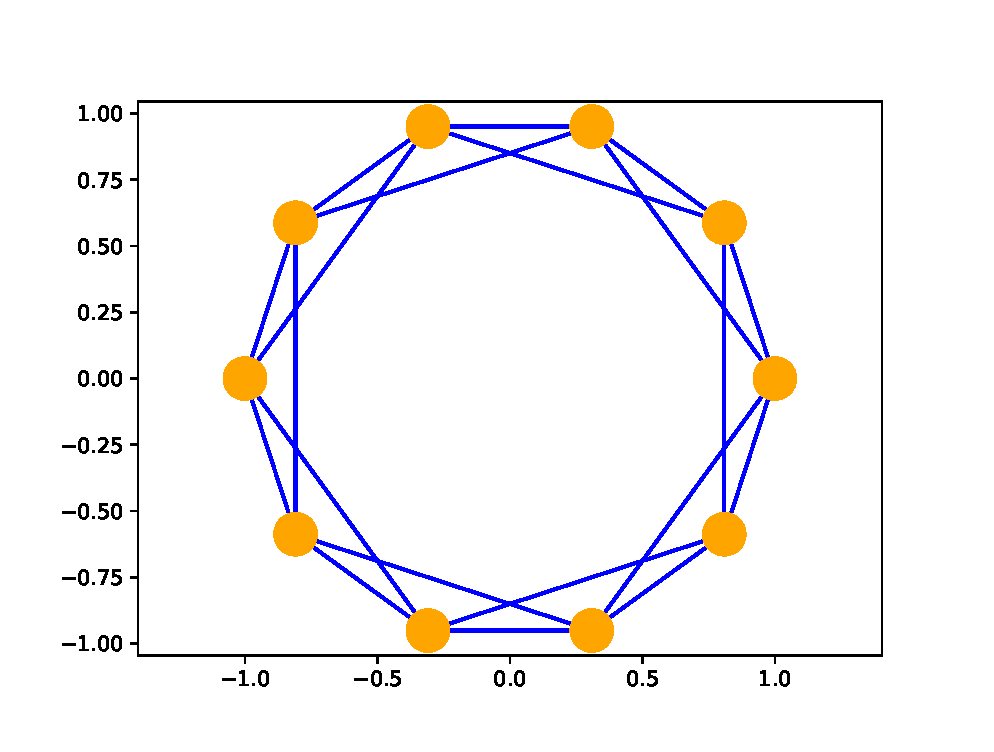
\includegraphics[scale=0.5]{WS_1.eps}
  \end{figure}
\end{frame}

\begin{frame}
  \frametitle{Algorithme de Watts-Strogatz}
  \begin{figure}[H]
    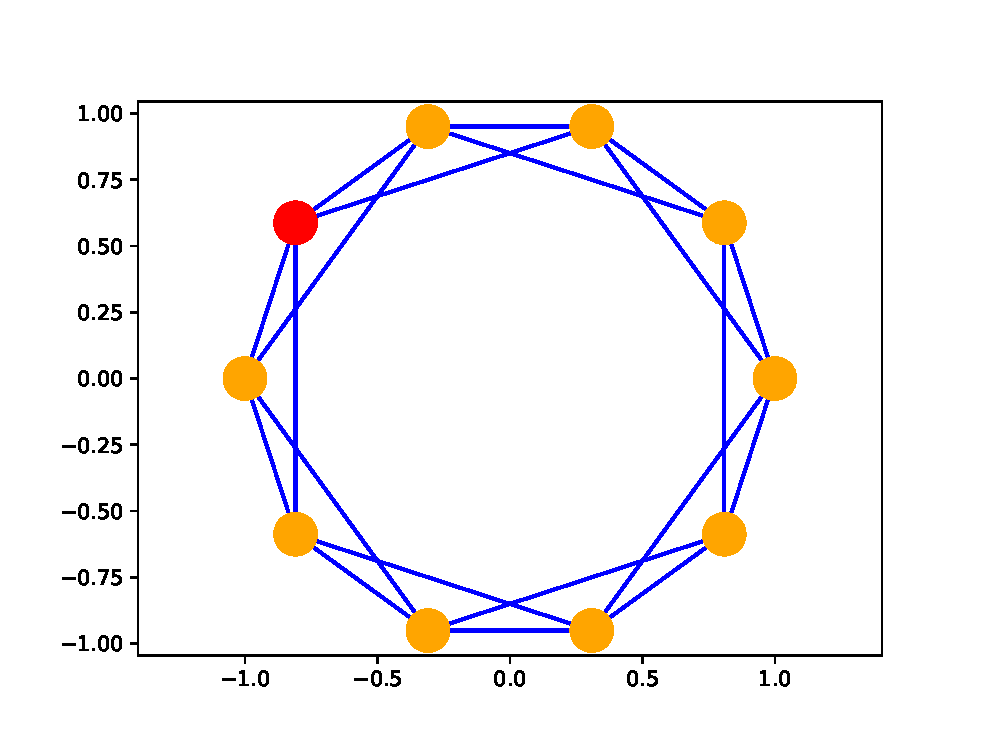
\includegraphics[scale=0.5]{WS_2.eps}
  \end{figure}
\end{frame}

\begin{frame}
  \frametitle{Algorithme de Watts-Strogatz}
  \begin{figure}[H]
    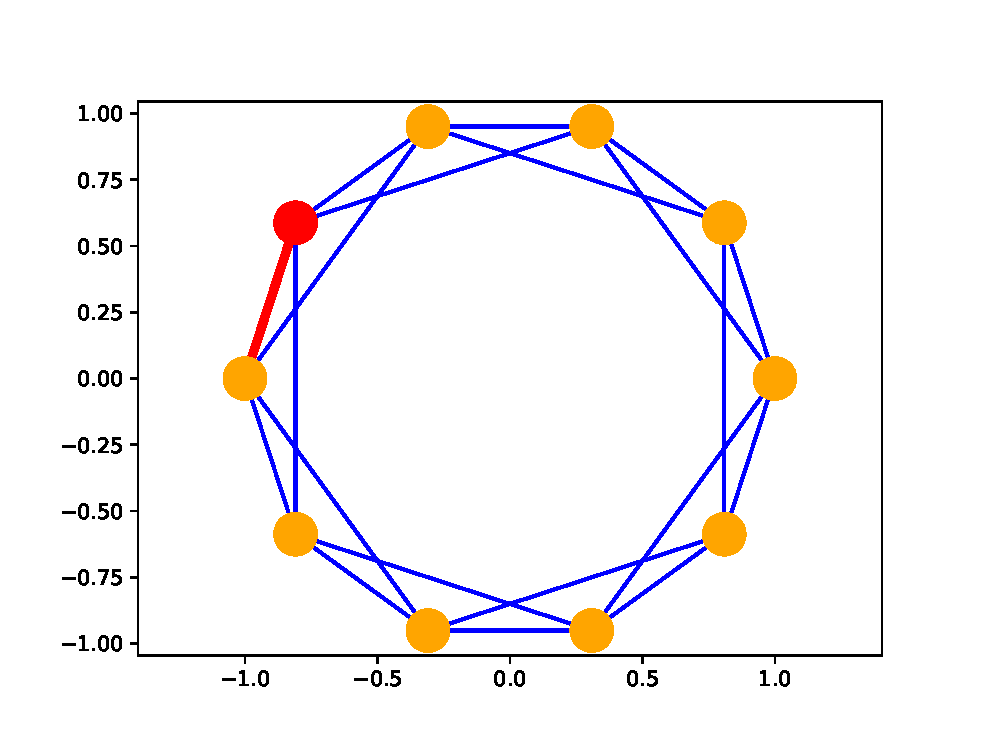
\includegraphics[scale=0.5]{WS_3.eps}
  \end{figure}
\end{frame}

\begin{frame}
  \frametitle{Algorithme de Watts-Strogatz}
  \begin{figure}[H]
    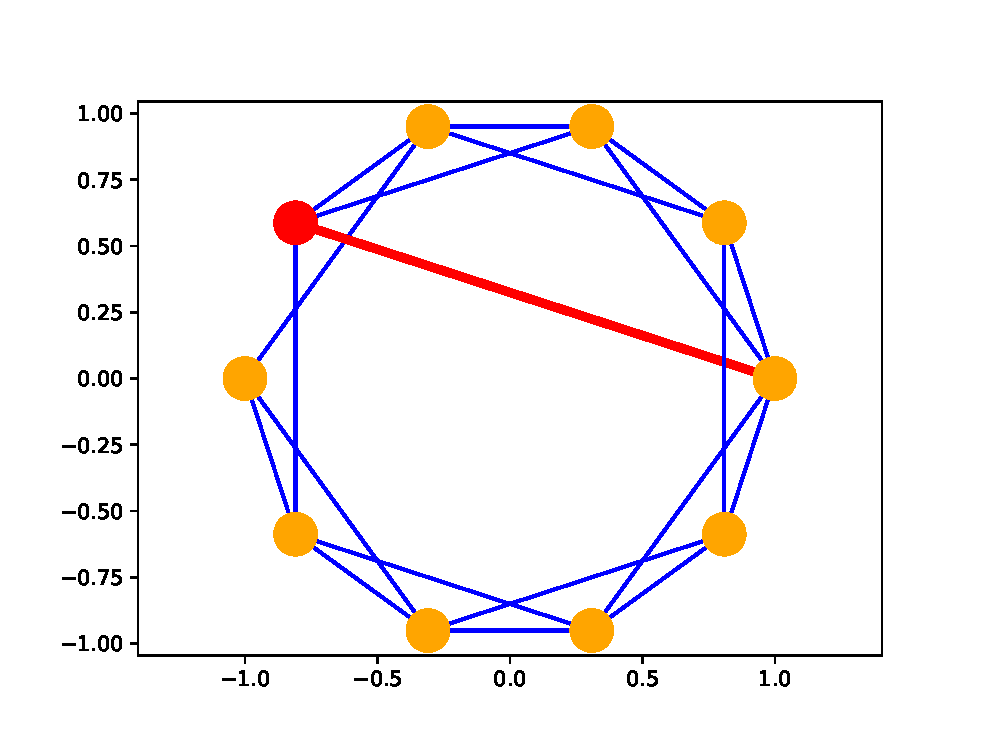
\includegraphics[scale=0.5]{WS_4.eps}
  \end{figure}
\end{frame}

\begin{frame}
  \frametitle{Algorithme de Watts-Strogatz}
  \begin{figure}[H]
    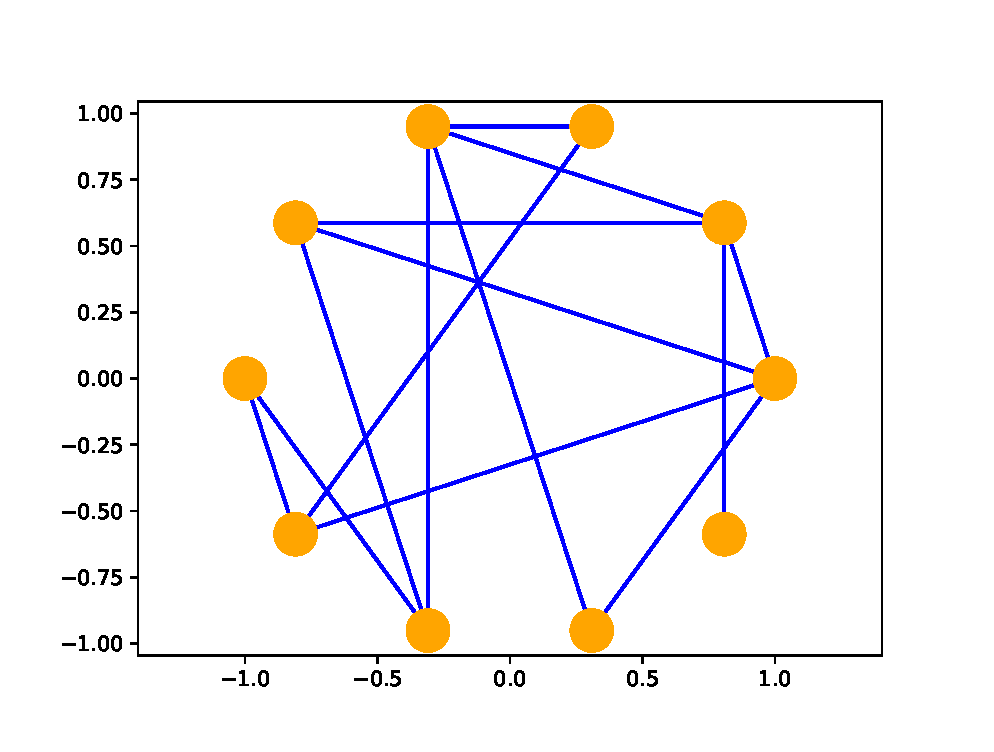
\includegraphics[scale=0.5]{WS_5.eps}
  \end{figure}
\end{frame}

\begin{frame}
  \frametitle{Réseaux simulés}
  \begin{itemize}
    \item<1-> 500 nœuds;
    \item<2-> Au plus 500 étapes de simulation;
    \item<3-> On lance la simulation 100 fois;
    \item<4-> 3 paramètres à examiner ($\beta$, $q$, proportion initiale d'informés)
  \end{itemize}
  \uncover<5->{
    $\rightarrow$ Stockage des résultats dans une base de donnée des résultats des calculs afin de pouvoir interrompre l'expérience à tout instant.
  }
\end{frame}

\section{Expérience 1}
\begin{frame}
  \frametitle{Protocole expérimental}
  On fixe $K=50$.
  Pour $\beta \in \{0,0.25,0.5,1\}$ et $q\in \{0.25, 0.5, 0.75\}$, pour une proportion initiale de 1\% à 99\% faire 100 expériences de propagation en choisissant les éléments initiaux au hasard et stocker la propagation à chaque étape de la simulation.

  \uncover<2->{
    But : pouvoir comparer les résultats des autres expériences, éventuellement fixer certains paramètres qui ont peu d'influence.
  }
\end{frame}

\subsection{Courbes de propagation}

\subsection{Proportion atteinte en fonction de la proportion initiale}
\begin{frame}
  \frametitle{Courbe type}
  \begin{figure}[H]
  \begin{center}
    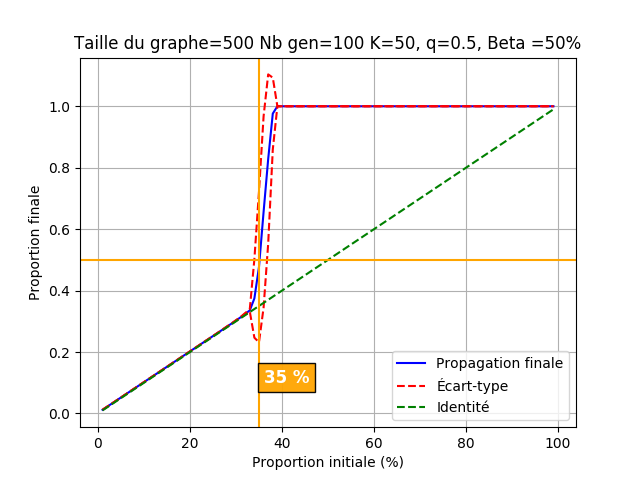
\includegraphics[width=\textwidth, height=0.8\textheight, keepaspectratio]{resultats/random_finale_f_initiale_q50_Beta50_ec.png}
  \end{center}
  \end{figure}
\end{frame}

\begin{frame}
  \frametitle{Faible influence du paramètre $\beta$}
  \only<1-1> {
  \begin{figure}[H]
  \begin{center}
    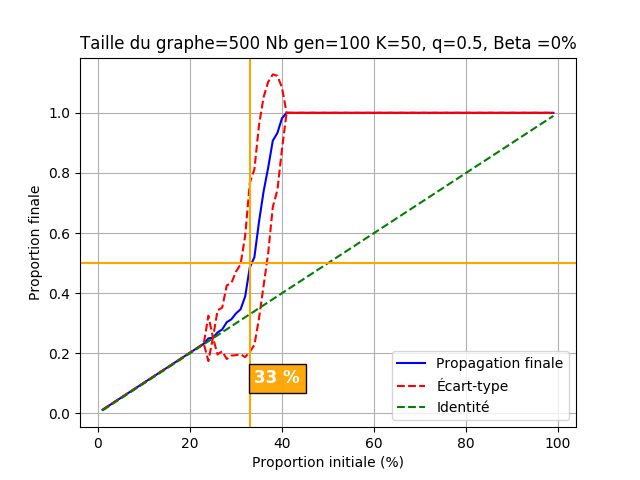
\includegraphics[width=\textwidth, height=0.8\textheight, keepaspectratio]{resultats/random_finale_f_initiale_q50_Beta0_ec.png}
  \end{center}
  \end{figure}
  }
  \only<2-2> {
  \begin{figure}[H]
  \begin{center}
    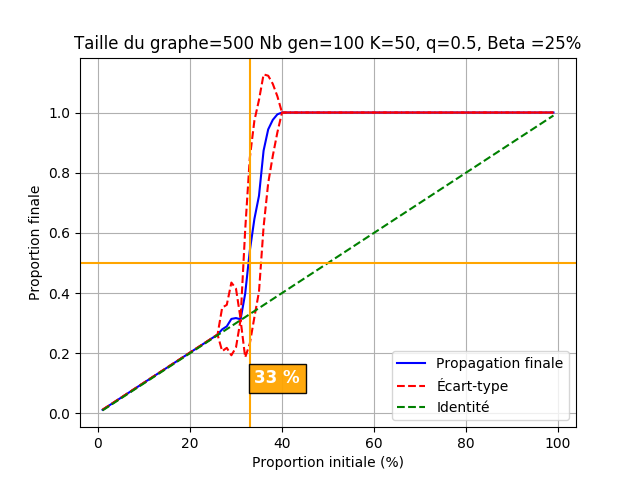
\includegraphics[width=\textwidth, height=0.8\textheight, keepaspectratio]{resultats/random_finale_f_initiale_q50_Beta25_ec.png}
  \end{center}
  \end{figure}
  }
  \only<3-3> {
  \begin{figure}[H]
  \begin{center}
    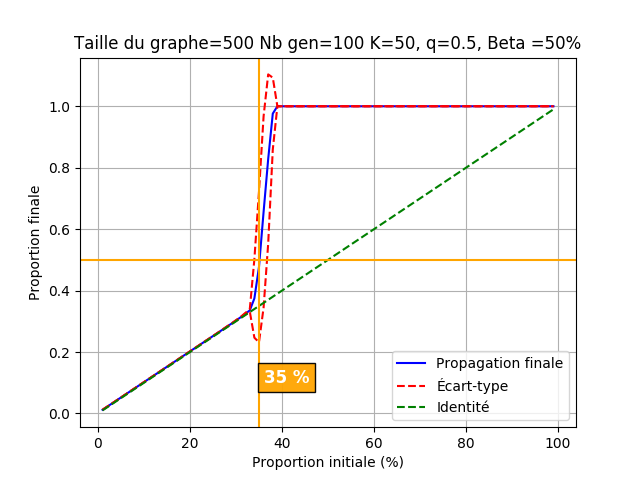
\includegraphics[width=\textwidth, height=0.8\textheight, keepaspectratio]{resultats/random_finale_f_initiale_q50_Beta50_ec.png}
  \end{center}
  \end{figure}
  }
  \only<4-4> {
  \begin{figure}[H]
  \begin{center}
    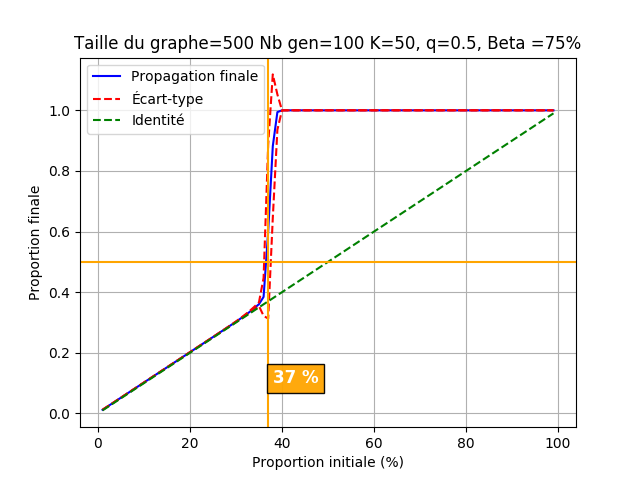
\includegraphics[width=\textwidth, height=0.8\textheight, keepaspectratio]{resultats/random_finale_f_initiale_q50_Beta75_ec.png}
  \end{center}
  \end{figure}
  }
  \only<5-5> {
  \begin{figure}[H]
  \begin{center}
    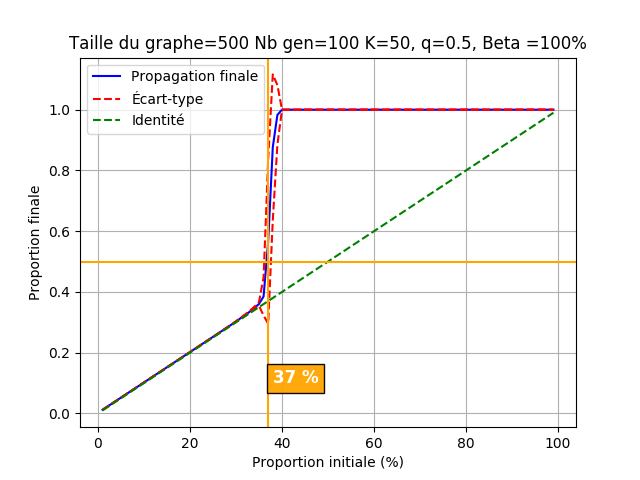
\includegraphics[width=\textwidth, height=0.8\textheight, keepaspectratio]{resultats/random_finale_f_initiale_q50_Beta100_ec.png}
  \end{center}
  \end{figure}
  }
\end{frame}

\begin{frame}
  \frametitle{Influence de $q$}
  \only<1-1>{
  \begin{figure}[H]
  \begin{center}
    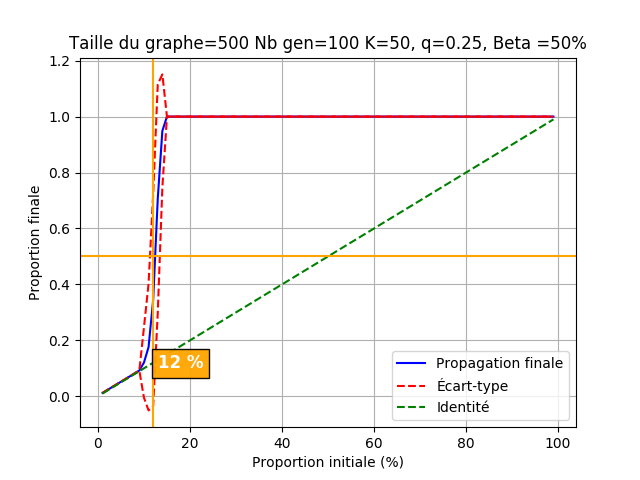
\includegraphics[width=\textwidth, height=0.8\textheight, keepaspectratio]{resultats/random_finale_f_initiale_q25_Beta50_ec.png}
  \end{center}
  \end{figure}
  }
  \only<2-2>{
  \begin{figure}[H]
  \begin{center}
    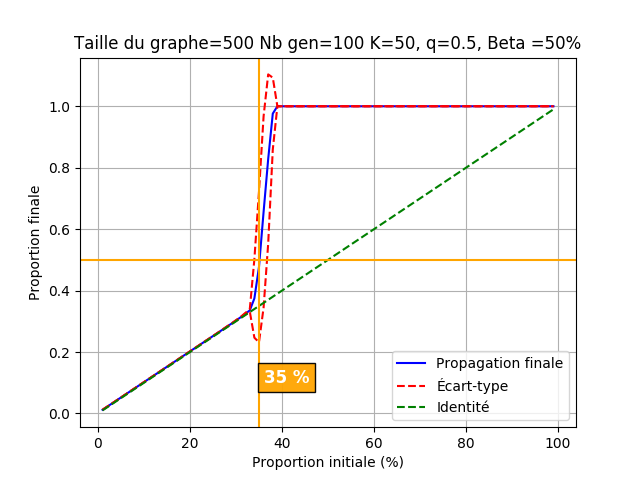
\includegraphics[width=\textwidth, height=0.8\textheight, keepaspectratio]{resultats/random_finale_f_initiale_q50_Beta50_ec.png}
  \end{center}
  \end{figure}
  }
  \only<3-3>{
  \begin{figure}[H]
  \begin{center}
    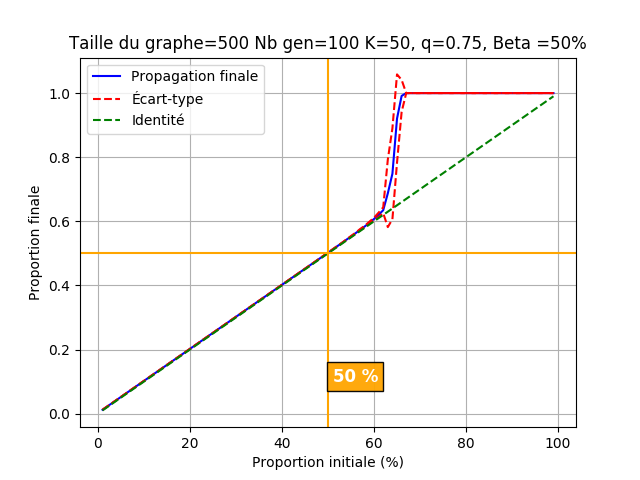
\includegraphics[width=\textwidth, height=0.8\textheight, keepaspectratio]{resultats/random_finale_f_initiale_q75_Beta50_ec.png}
  \end{center}
  \end{figure}
  }
  % \begin{figure}[H]
  % \begin{center}
    % 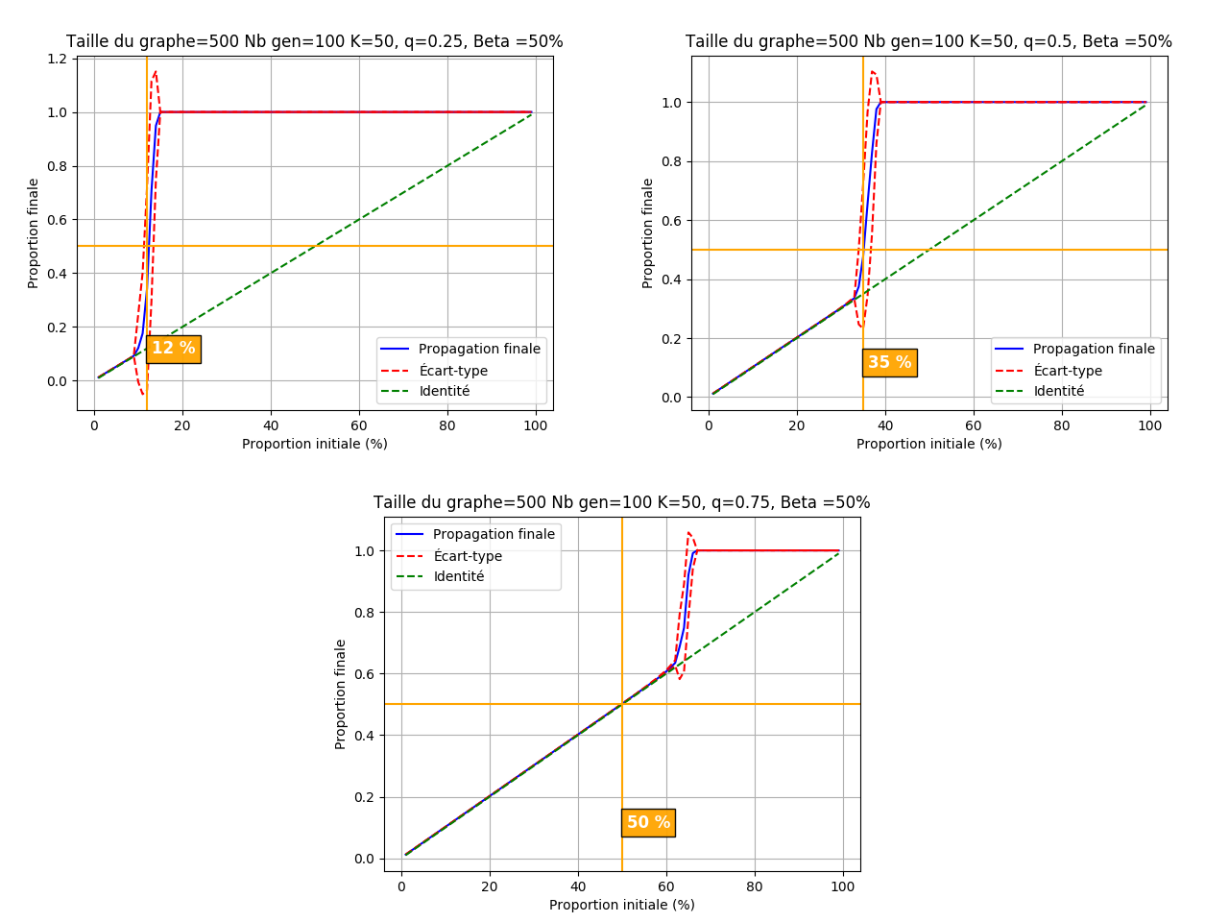
\includegraphics[width=\textwidth, height=0.8\textheight, keepaspectratio]{resultats/comp_random_beta50.png}
  % \end{center}
  % \end{figure}
\end{frame}

\section{Expérience 2}
\begin{frame}
  \frametitle{Protocole expérimental}
  On fixe $K=50$.
  Pour $\beta \in \{0,0.25,0.5,1\}$ et $q\in \{0.25, 0.5, 0.75\}$, pour une proportion initiale de 1\% à 99\% faire 100 expériences de propagation en choisissant les éléments initiaux possèdant la plus grande arité et stocker la propagation à chaque étape de la simulation.
\end{frame}
\begin{frame}
  \frametitle{Remarques sur les résultats}
  \begin{itemize}
    \item<1-> Le résultat pour $\beta=0$ est inexploitable;
    \item<2-> On retrouve les mêmes effets qualitatifs de $\beta$ et $q$.
  \end{itemize}
\end{frame}

\section{Expérience 3}
\begin{frame}
  \frametitle{Protocole expérimental}
  On fixe $K=50$.
  Pour $\beta \in \{0,0.25,0.5,1\}$ et $q\in \{0.25, 0.5, 0.75\}$, pour une proportion initiale de 1\% à 99\% faire 100 expériences de propagation en choisissant les éléments initiaux possèdant la plus grande centralité (proportion de plus courts chemins passants par un nœud) et stocker la propagation à chaque étape de la simulation.
\end{frame}
\begin{frame}
  \frametitle{Remarques sur les résultats}
  \begin{itemize}
    \item<1-> Le résultat pour $\beta=0$ est inexploitable;
    \item<2-> On retrouve les mêmes effets qualitatifs de $\beta$ et $q$.
  \end{itemize}
\end{frame}

\section{Résultats}
\subsection{Comparaison}
\subsection{Conséquences}

\section{Conclusion}


\end{document}